\documentclass{standalone}
\usepackage{tikz}
\begin{document}
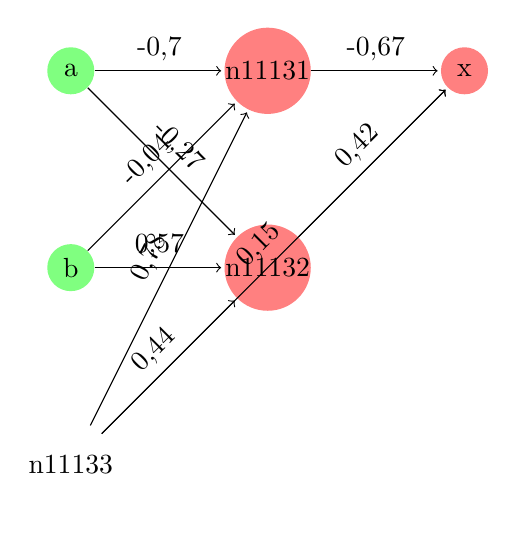
\begin{tikzpicture}[shorten >=1pt,->,draw=black!,node distance=2.5cm]
\tikzstyle{neuron}=[circle,fill=black!25,minimum size=17pt,inner sep=0pt]
\tikzstyle{constant}=[neuron, fill=white!50];
\tikzstyle{sigmoid}=[neuron, fill=red!50];
\tikzstyle{identity}=[neuron, fill=green!50];
\node [identity] (a) {a};
\node [identity,below of=a] (b) {b};
\node [constant,below of=b] (n11133) {n11133};
\node [sigmoid,right of=a] (n11131) {n11131};
\node [sigmoid,below of=n11131] (n11132) {n11132};
\node [sigmoid,right of=n11131] (x) {x};
\path[every node/.style={sloped,anchor=south,auto=false}]
(n11133) edge node {0,15} (x)
(n11133) edge node {0,44} (n11132)
(n11133) edge node {0,78} (n11131)
(n11131) edge node {-0,67} (x)
(n11132) edge node {0,42} (x)
(a) edge node {-0,7} (n11131)
(a) edge node {-0,27} (n11132)
(b) edge node {-0,04} (n11131)
(b) edge node {0,57} (n11132)
;\end{tikzpicture}
\end{document}